\documentclass[colorlinks]{beamer}

\usepackage[utf8]{inputenc}
\usepackage{fancybox}
\usepackage{environ,fancyvrb,tikz}

\newcommand{\ds}{\displaystyle}
\newcommand{\grad}{\nabla}
\newcommand{\ih}{\boldsymbol{\hat{\textbf{\i}}}}
\newcommand{\jh}{\boldsymbol{\hat{\textbf{\j}}}}
\newcommand{\vF}{\boldsymbol{\vec{\textbf{F}}}}

\newcommand\enumnum[1]{{\renewcommand{\insertenumlabel}{#1}%
      \usebeamertemplate{enumerate item} \,}}

\beamertemplatenavigationsymbolsempty


\title{3.2 Nonlinear Models}

\subtitle{a lecture for MATH F302 Differential Equations}

\author{Ed Bueler, Dept.~of Mathematics and Statistics, UAF}

\date{Fall 2023}


\usetheme{Pittsburgh}


\begin{document}

\setbeamertemplate{itemize item}{$\bullet$}
\setbeamertemplate{itemize subitem}{$\circ$}


\begin{frame}
\titlepage

\centerline{\tiny for textbook: \, D. Zill, \emph{A First Course in Differential Equations with Modeling Applications}, 11th ed.}
\end{frame}


\begin{frame}{outline}

\begin{itemize}
\item like 3.1, section 3.2 has modeling problems
    \begin{itemize}
    \item \emph{challenging} modeling problems
    \item uses separable equations from \S2.2: $\frac{dy}{dx} = g(x) h(y)$
    \end{itemize}
\item plan for these slides:
    \begin{itemize}
    \item start with five standard indefinite integrals
        \begin{itemize}
        \item you did them in calculus I and II
        \item \dots but a reminder is appropriate
        \end{itemize}
    \item two explanations of where the ``logistic equation'' comes from
    \item solve the logistic equation
    \item two exercises from \S3.2
    \end{itemize} 
\end{itemize}
\end{frame}


\begin{frame}{integrals you will need}

\begin{itemize}
\item {\color{blue} integral 1} was already used in \S3.1:
    $$\int \frac{dy}{ay+b} = \hspace{80mm}$$

\vspace{10mm}
\item {\color{blue} integral 2} is sometimes useful:
    $$\int \frac{dx}{x^2+a^2} = \hspace{80mm}$$

\vspace{25mm}
\end{itemize}
\end{frame}


\begin{frame}{integrals, cont.}

\begin{itemize}
\item {\color{blue} integral 3} is the main job in \S3.2:
    $$\int \frac{dz}{z(a-bz)} = \hspace{80mm}$$

\vspace{50mm}
\end{itemize}
\end{frame}


\begin{frame}{integrals, cont.$^2$}

\begin{itemize}
\item {\color{blue} integral 4} was needed for first-order linear equations (\S2.3) and will keep re-appearing in chapter 4 and onward:
    $$\int x^n e^{ax}\,dx = \hspace{80mm}$$

\vspace{30mm}

$$\int x e^x\,dx = \hspace{80mm}$$

$$\int_0^\infty x^2 e^{-x}\,dx = \hspace{80mm}$$
\end{itemize}
\end{frame}


\begin{frame}{integrals, cont.$^3$}

\begin{itemize}
\item {\color{blue} integral 5} will keep re-appearing in chapter 4 and onward:
    $$\int e^{at} \cos bt\,dt = \hspace{80mm}$$

\vspace{60mm}
\end{itemize}
\end{frame}


\begin{frame}{how to remember integrals}

\begin{itemize}
\item even if you have a good memory, I think it is silly to try to rawly memorize the \emph{results} above
\item but \emph{do}
    \begin{itemize}
    \item try to remember what choices which were made, and \emph{why}
    \item remember how to start partial fractions
    \item think of integration-by-parts as undoing the product rule
    \item $\int x^n e^{ax}\,dx$: integration-by-parts gives a reduction formula
    \item $\int e^{at} \cos bt\,dt$: there is a double integration-by-parts trick
    \end{itemize}
\end{itemize}
\end{frame}


\begin{frame}{logistic equation: explanation 1}

\small
\begin{quotation}
\noindent Suppose we have a dish with no bacteria, and we plan to supply enough food and water every hour to sustain the needs of $N$ bacteria.  Question: What will happen when we introduce a few bacteria ($P_0 \ll N$)?
\end{quotation}

\normalsize
\begin{itemize}
\item \emph{model we know}:  $P(t)$ is population, $P(0)=P_0$, $k>0$,
    $$\frac{dP}{dt} = k P$$

\vspace{-2mm}
    \begin{itemize}
    \item has solution $P(t) = P_0 e^{kt}$
    \item predicts unlimited exponential growth
    \item at some point population growth in dish will be limited by food and water
    \end{itemize}
\item \emph{better model}: make coefficient get smaller as $P$ gets larger
    $$\frac{dP}{dt} = \left(\begin{matrix} \text{coefficient which gets} \\ \text{smaller when $P$ approaches $N$}\end{matrix} \right) P$$
\end{itemize}
\end{frame}


\begin{frame}{explanation 1, cont.}

\begin{itemize}
\item a formula with the desired property:
    $$\boxed{\frac{dP}{dt} = k \left(1-\frac{P}{N}\right) P} \hspace{50mm}$$
\item equivalently with $b=k/N >0$:
    $$\boxed{\frac{dP}{dt} = b P \left(N-P\right)} \hspace{50mm}$$
\item previous model was linear; this one is nonlinear
     \begin{itemize}
     \item but separable!
     \end{itemize}
\end{itemize}
\end{frame}


\begin{frame}{explanation 1, cont.$^2$}

\begin{itemize}
\item a formula with the desired property: $\ds \frac{dP}{dt} = b P \left(N-P\right)$, $b>0$
\item draw phase portrait and typical solutions
\end{itemize}

\vspace{50mm}
\end{frame}


\begin{frame}{logistic equation: explanation 2}

\small
\begin{quotation}
\noindent Suppose a population changes by two mechanisms, namely births (rate is proportional to current population) and deaths by conflicts between the members of the population (rate is proportional to number of interactions, modeled as the square of the population).
\end{quotation}

\normalsize
\begin{itemize}
\item write down the DE, with constants $k>0$ and $\ell>0$:
    $$\boxed{\frac{dP}{dt} = k P - \ell P^2}$$
\item equivalently, using $b=\ell$ and $N=k/\ell$, again write as $\frac{dP}{dt} = b P \left(N-P\right)$
\item look at the last three boxed equations
    \begin{itemize}
    \item they are all called the \emph{logistic equation}
    \item the three forms are equivalent by renaming the constants
    \end{itemize}
\end{itemize}
\end{frame}


\begin{frame}{logistic equation: solve}

\begin{itemize}
\item assuming $a,b$ are positive constants, find the general solution:
    $$\frac{dP}{dt} = P \left(a - bP\right) \hspace{70mm}$$
\end{itemize}

\vspace{50mm}
\end{frame}


\begin{frame}{logistic equation: verify solution}

\begin{itemize}
\item show that
    $$P(t)=\frac{aP_0}{bP_0+(a-bP_0) e^{-at}}$$
solves $\frac{dP}{dt} = P \left(a-bP\right)$ and $P(0)=P_0$
\end{itemize}

\vspace{50mm}
\end{frame}


\begin{frame}[fragile]

\frametitle{exercise 4 in \S3.2}

\small
\begin{quotation}
\noindent Census data for the United States between 1790 and 1950 are given in the Table on page 102.  (a)   Construct a logistic population model using the data from 1790, 1850, and 1910.  (b)  Show a plot comparing actual census population with the population predicted by the model.
\end{quotation}

\normalsize
\begin{itemize}
\item first I put the Table in a Matlab code and plotted it

\medskip
\begin{Verbatim}[fontsize=\footnotesize,xleftmargin=7mm]
year = 1790:10:1950;    % list of 17 values
pop = [  3.929,   5.308,   7.240,   9.638,  12.866, ...
        17.069,  23.192,  31.433,  38.558,  50.156, ...
        62.948,  75.996,  91.972, 105.711, 122.775, ...
       131.669, 150.697];
plot(year, pop, '.k')
xlabel('census year')
ylabel('population in millions')
axis([1780 1960 0 160]),  grid on
\end{Verbatim}
\end{itemize}
\end{frame}


\begin{frame}{exercise 4, cont.}

\begin{center}
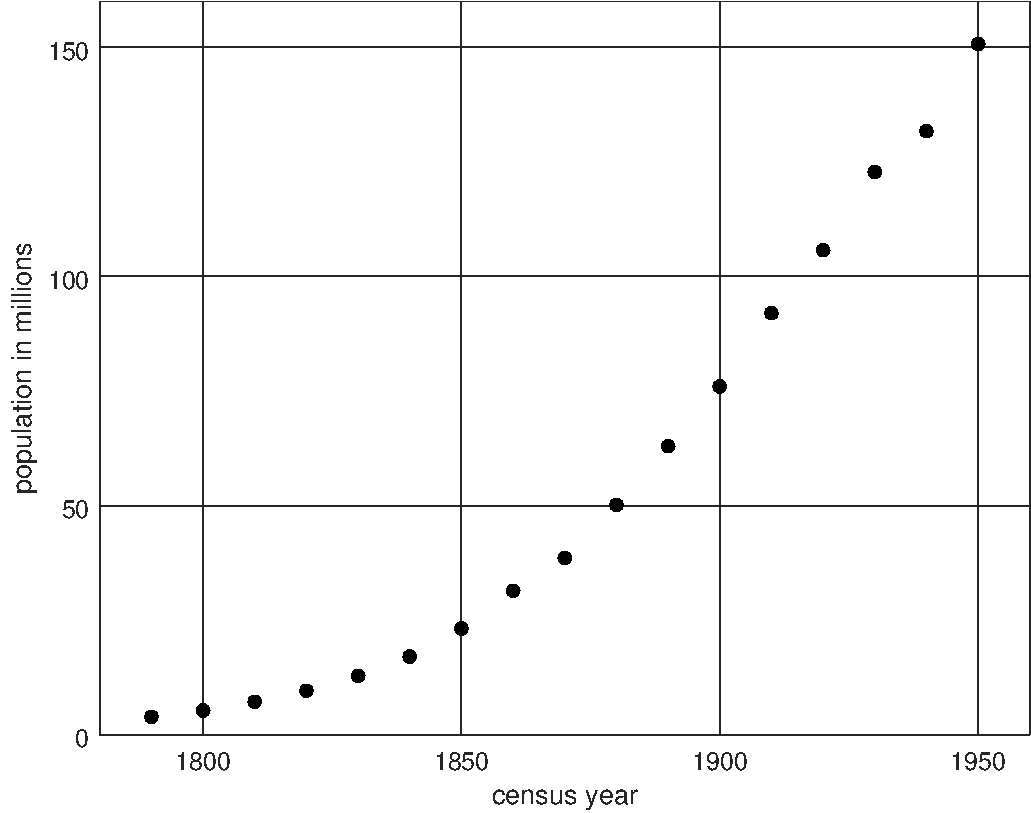
\includegraphics[width=0.75\textwidth]{figs/plotcensus}
\end{center}
\end{frame}


\begin{frame}{exercise 4, cont.$^2$}

\begin{itemize}
\item we are supposed to construct a logistic model using the 1790, 1850, 1910 populations
\item we use those years to determine $P_0,a,b$ in
$$P(t)=\frac{aP_0}{bP_0+(a-bP_0) e^{-at}} = \frac{a}{b+(a/P_0-b) e^{-at}}$$
\item let $t$ be number of years after 1790: $P_0=3.929$ (millions)
\item now 2 equations in 2 unknowns $a,b$ from $P(60)=23.192$ and $P(120)=91.972$:
\small
\begin{align*}
23.192 &= \frac{a}{b+(a/3.929-b) e^{-60a}} \\
91.972 &= \frac{a}{b+(a/3.929-b) e^{-120a}}
\end{align*}
\normalsize
\item this algebra job is hard!
\end{itemize}
\end{frame}


\begin{frame}[fragile]

\frametitle{exercise 4, cont.$^2$}

\noindent \textbf{Problem.}  Solve 2 equations in 2 unknowns $a,b$:
\small
\begin{align*}
23.192 &= \frac{a}{b+(a/3.929-b) e^{-60a}} \\
91.972 &= \frac{a}{b+(a/3.929-b) e^{-120a}}
\end{align*}

\noindent \textbf{My solution.}  I typed into \texttt{wolframalpha.com}:

\begin{Verbatim}[fontsize=\footnotesize,xleftmargin=7mm]
solve: 23.192 = a / (b + (a/3.929 - b) e^(-60a)),
       91.972 = a / (b + (a/3.929 - b) e^(-120a))
\end{Verbatim}

It gave me one \emph{real} answer:
	$$a = 0.0313395, b = 0.000158863$$

\bigskip
\begin{itemize}
\item checking: with our values of $P_0,a,b$ it returns $P(60)=23.192$ and $P(120)=91.972$.

\item on the next slide I plot $P(t)$ in red on top of the data; the fit is surprisingly good!
\end{itemize}
\end{frame}


\begin{frame}{exercise 4, finished}

\begin{center}
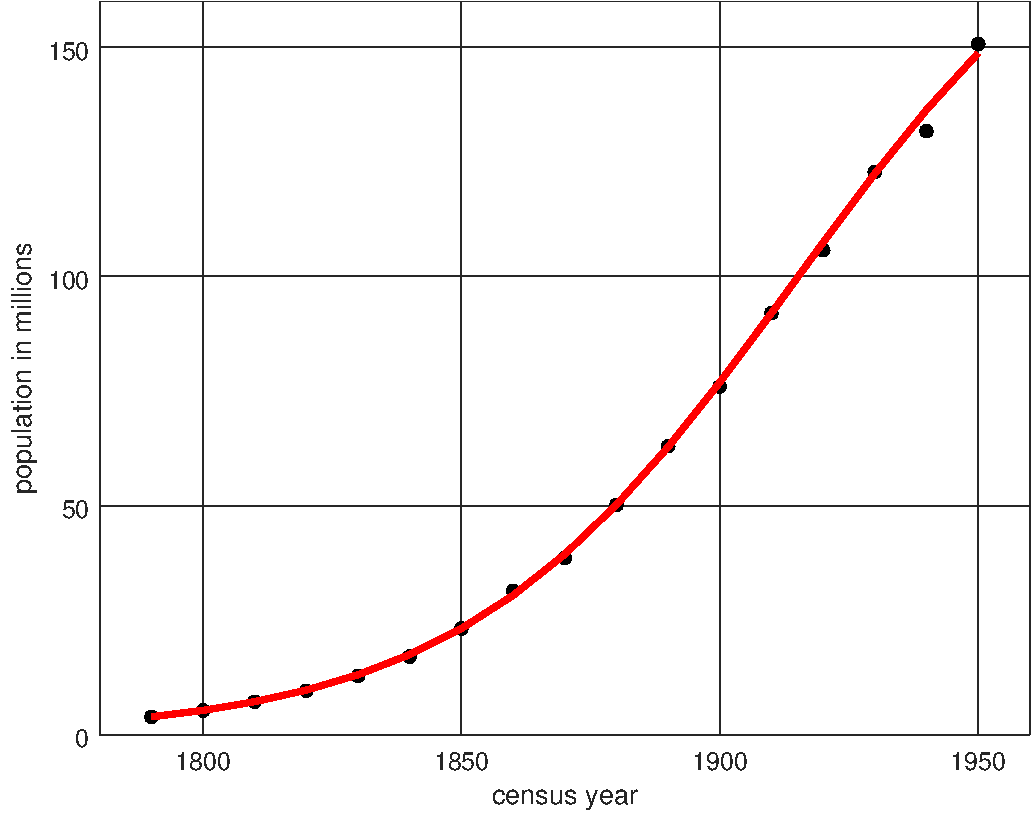
\includegraphics[width=0.6\textwidth]{figs/fitcensus}
\end{center}

\vspace{-2mm}
\begin{itemize}
\item in our model:
    $$\lim_{t\to \infty} P(t) = \lim_{t\to \infty} \frac{a}{b+(a/P_0-b) e^{-at}} = \frac{a}{b} = 197 \text{ million}$$
\item in fact the current US population is definitely larger than that, about 328 million at the start of 2019
\end{itemize}
\end{frame}


\begin{frame}{exercise 15 in \S3.2}

\begin{quotation}
\noindent \textbf{Air Resistance} \, A DE for the velocity $v$ of a falling mass $m$ subjected to air resistance proportional to the \underline{square} of the velocity is
    $$m \frac{dv}{dt} = m g - k v^2$$
where $k>0$ and the positive direction is downward.

(a) Solve the equation subject to $v(0)=v_0$.

(b) Determine the terminal velocity.  Compare to a phase portrait of the DE.
\end{quotation}

\begin{itemize}
\item note $m>0$ and $g>0$
\item my first step is to simplify by dividing by $m$ and factoring $g$:
    $$\frac{dv}{dt} = g - \frac{k}{m} v^2 = g \left(1 - \frac{k}{mg} v^2\right)$$
\item let $R=\sqrt{k/(mg)}$ to get form: $\frac{dv}{dt} = g \left(1 - R^2 v^2\right)$
\end{itemize}
\end{frame}


\begin{frame}{exercise 15, cont.}

\begin{itemize}
\item from last slide we want to solve:
   $$\frac{dv}{dt} = g \left(1 - R^2 v^2\right) \quad \text{ where } R=\sqrt{\frac{k}{mg}}$$
\end{itemize}

\vspace{60mm}
\end{frame}


\begin{frame}{exercise 15, finished}

\begin{quotation}
\noindent (b) Determine the terminal velocity.  Compare to a phase portrait of the DE.
\end{quotation}

\vspace{60mm}
\end{frame}


\begin{frame}{expectations}

\begin{itemize}
\item to learn this material, just listening to a lecture is \emph{not} enough!
\item \emph{read} section 3.2 in the textbook
    \begin{itemize}
    \item \emph{read} example 2 on pages 100--101 regarding a chemical equation
    \item look for ``logistic differential equation'' on YouTube or Google
    \item do you actually know how to do the integrals at the start of these slides?
    \item do Homework 3.2
    \end{itemize}
\item up next are second-order linear equations in section 4.1
    \begin{itemize}
    \item for now we skip section 3.3
    \item we will return to it near the end of the course, linking it with material in chapter 8
    \end{itemize}
\end{itemize}
\end{frame}


\end{document}

